\documentclass{classrep}
\usepackage[utf8]{inputenc}
\frenchspacing

\usepackage{graphicx}
\usepackage[usenames,dvipsnames]{color}
\usepackage[hidelinks]{hyperref}

\usepackage{amsmath, amssymb, mathtools}

\usepackage{fancyhdr, lastpage}
\pagestyle{fancyplain}
\fancyhf{}
\renewcommand{\headrulewidth}{0pt}
\cfoot{\thepage\ / \pageref*{LastPage}}
\newcommand{\R}{\mathbb{R}}

\studycycle{Informatyka, studia dzienne, I st.}
\coursesemester{IV}

\coursename{Sztuczna inteligencja i systemy eskpertowe}
\courseyear{2018/2019}

\courseteacher{dr inż. Krzysztof Lichy}
\coursegroup{piątek, 08:30}

\author{%
  \studentinfo[210139@edu.p.lodz.pl]{Krzysztof Barden}{210139}
}

\title{Zadanie 2.: Sieć neuronowa - Perceptron wielowarstwowy}

\begin{document}
\maketitle
\thispagestyle{fancyplain}

\section{Cel}
{
Zadanie polega na napisaniu programu implementującego sieć neuronową typu wielowarstwowy perceptron, nauczaną metodą wstecznej propagacji błędu.
Sieć neuronowa ma zostać nauczona obliczania pierwiastka drugiego stopnia liczby przez użycie wejsciowego wektora liczb losowych z zakresu 1-100/

}

\section{Wprowadzenie}
{
Perceptron wielowarstwowy – najpopularniejszy typ sztucznych 
sieci neuronowych. Sieć tego typu składa się zwykle z jednej warstwy
 wejściowej, kilku warstw ukrytych oraz jednej warstwy wyjściowej.\\
Perceptron wielowarstwowy w przeciwieństwie do perceptronu jednowarstwowego 
może być wykorzystywany do klasyfikowania zbiorów, które nie są liniowo separowalne.
Ogólny wzór opisujący perceptrony:
\begin{equation}
f_w : \R ^n \rightarrow \R ^m\\
\end{equation}
gdzie n to wejscia, w to wagi, m to wyjscia\\ 
W tym zadaniu perceptron wielowarstwowy jest uczony metodą wstecznej propagacji.}

\section{Opis implementacji}
{Do wykonania zadania został użyty język Python.\\\\
Sieć neuronowa(MLP) przyjmuje jako parametry ilosć wejsć (w tym zadaniu zawsze 1), ilosć neuronów w warstwie ukrytej, ilosć wyjsć (w tym zadaniu zawsze 1)
, współczynnik nauki, wspołczynnik momentum, wybór czy używać biasu, ilosć epok oraz wartosć próbkowania błędu.\\
Wartosći wag są inicjalizowane w przedziale <-0.5;0,5>.\\
Funkcją aktywacyjną jest funkcja sigmoidalna.\\
Sekwencja czynności, która zostaje wykonana przy nauce MLP: wzorzec treningowy podawany jest na wejścia sieci, następnie odbywa się jego propagacja wprzód, dalej na podstawie wartości odpowiedzi wygenerowanej przez sieć oraz wartości pożądanego wzorca odpowiedzi następuje wyznaczenie błędów, po czym propagowane są one wstecz, na koniec zaś ma miejsce wprowadzenie poprawek na wagi.\\
Sekwencja czynności przy testowaniu MLP: wzorzec treningowy podawany jest na wejścia sieci, następnie odbywa się jego propagacja wprzód, a na koniec na podstawie wartości odpowiedzi wygenerowanej przez sieć oraz wartości pożądanego wzorca odpowiedzi następuje wyznaczenie błędów.
}

\section{Materiały i metody}
{Na wejsciu podawany losowo przetasowany znormalizowany wektor liczb od 1 do 100.
Oczekiwane wyjscie to wartosci pierwiastka kwadratowego liczb z wejsciowego wektora.

Do ostatniego ekperymentu po nauczeniu sieci zadano wektor liczb od 1 do 150 w celu okreslenia możliwosci sieci do ekstrapolacji.
}
\section{Wyniki}
{
Podpunkt 1.1\\
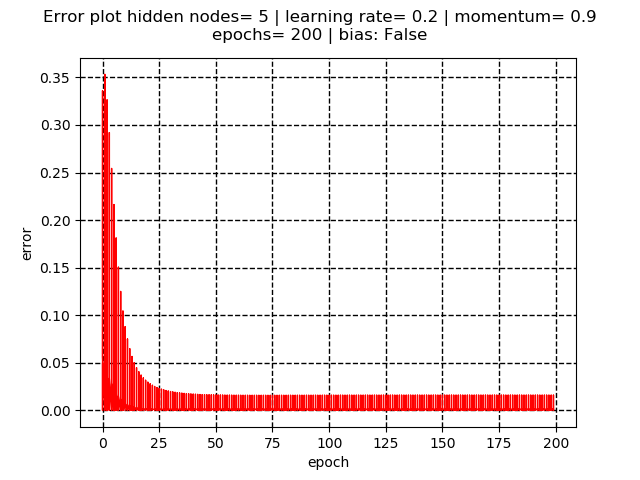
\includegraphics[scale=0.8]{imgs/1_1.png}\\
Podpunkt 1.2\\
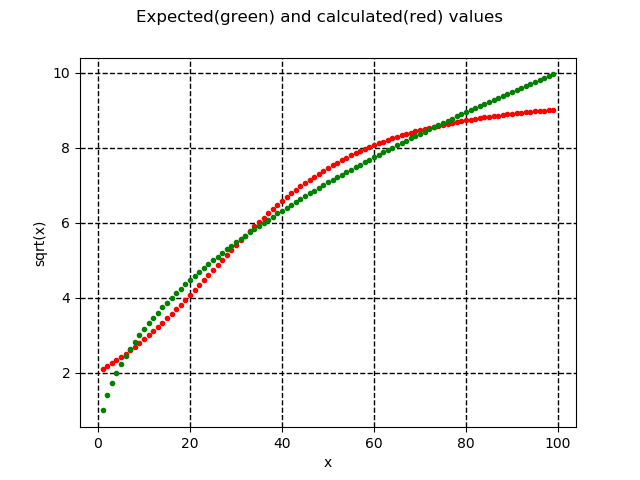
\includegraphics[scale=0.8]{imgs/1_2.png}\\
}  

{Eksperyment 2\\
Podpunkt 2.1\\
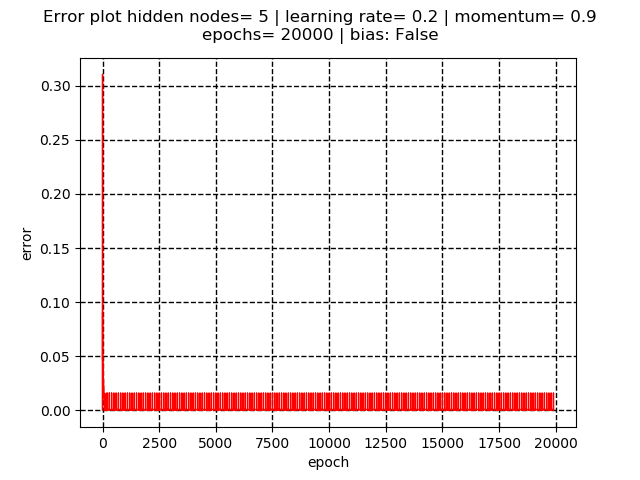
\includegraphics[scale=0.8]{imgs/2_1.png}\\
Podpunkt 2.2\\
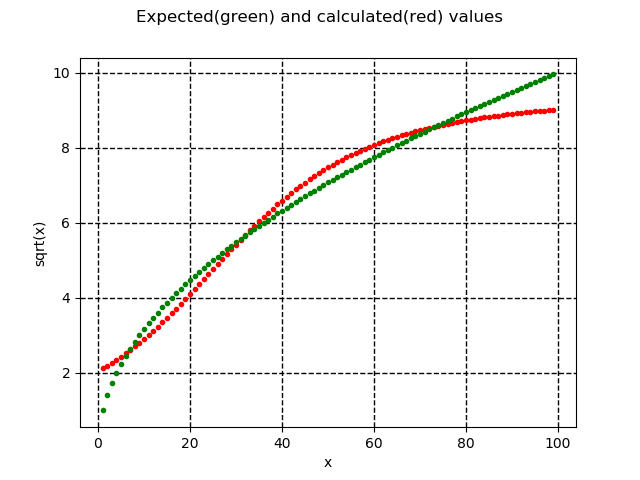
\includegraphics[scale=0.8]{imgs/2_2.png}\\
}

{Eksperyment 3\\
Podpunkt 3.1\\
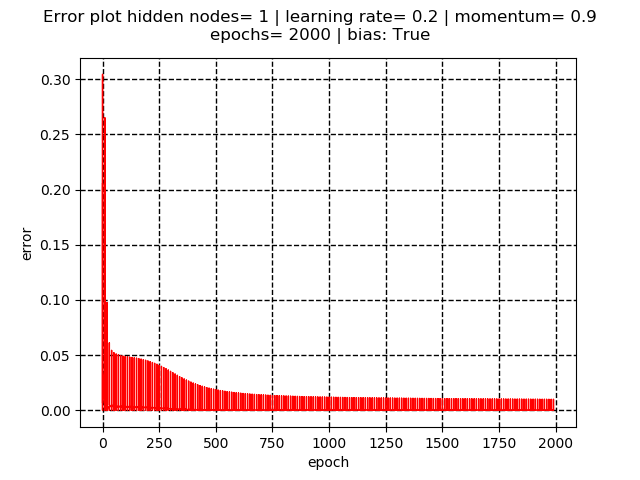
\includegraphics[scale=0.8]{imgs/3_1.png}\\
Podpunkt 3.2\\
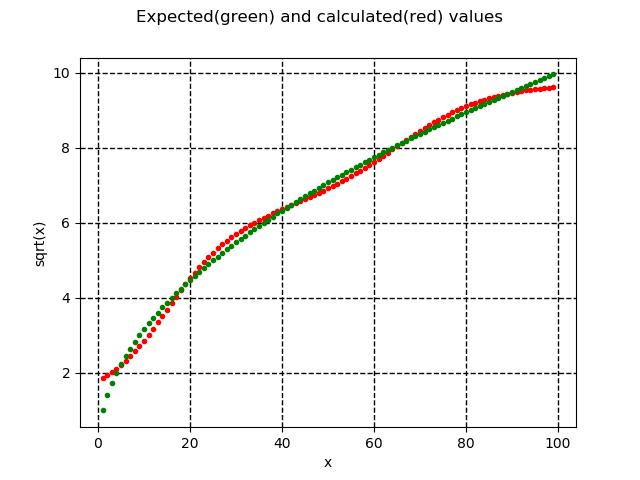
\includegraphics[scale=0.8]{imgs/3_2.png}\\
}

{Eksperyment 4\\
Podpunkt 4.1\\
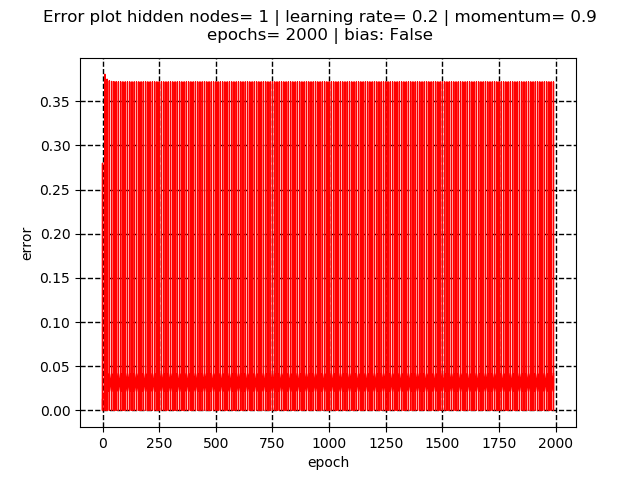
\includegraphics[scale=0.8]{imgs/4_1.png}\\
Podpunkt 4.2\\
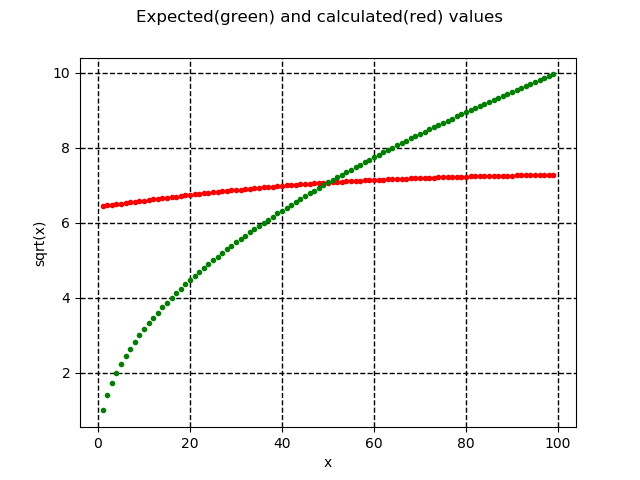
\includegraphics[scale=0.8]{imgs/4_2.png}\\
}


{Eksperyment 5\\
Podpunkt 5.1\\
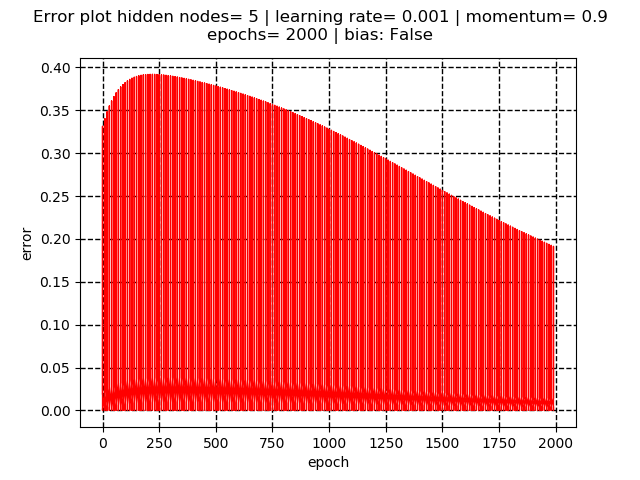
\includegraphics[scale=0.8]{imgs/5_1.png}\\
Podpunkt 5.2\\
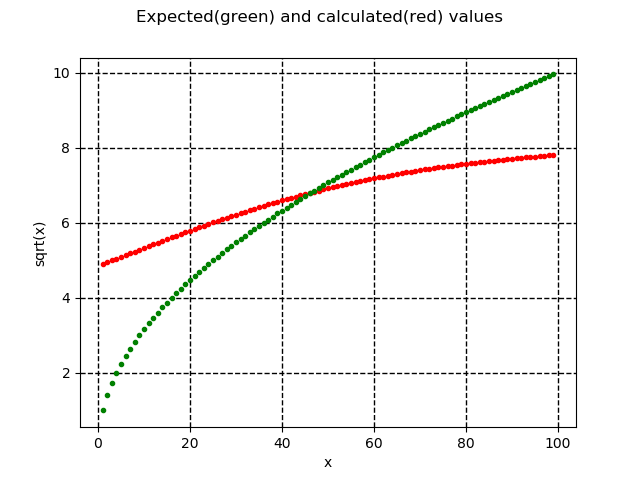
\includegraphics[scale=0.8]{imgs/5_2.png}\\

{Eksperyment 6\\
Podpunkt 6.1\\
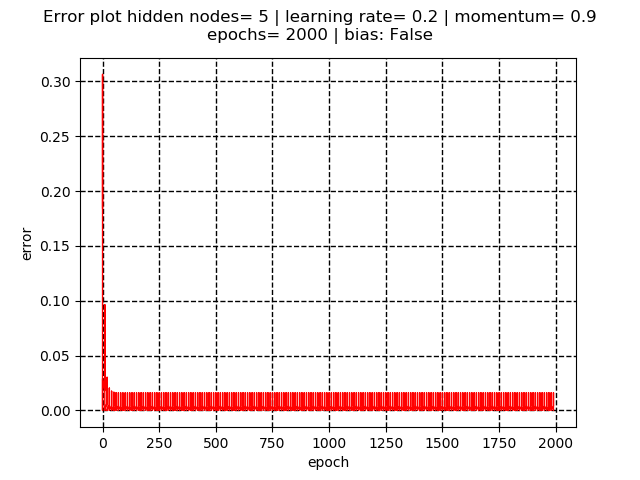
\includegraphics[scale=0.8]{imgs/longer1.png}\\
Podpunkt 6.2\\
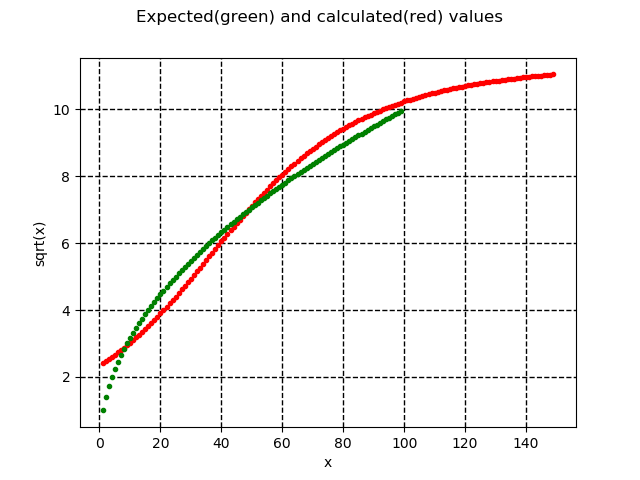
\includegraphics[scale=0.8]{imgs/longer2.png}\\


}




\section{Dyskusja}
{
Zwiększając ilosć epok nie zawsze sie zwiększa dokładnosć, może wystąpić przetrenowanie lub zmiany będą zbyt małe do zauważenia.\\
Dobranie learning rate ma duże znaczenie. 
Zbyt duże wartosci mogą doprowadzać do powstawania większych błędów, ale zbyt małe spowalniają proces nauki.\\
Zbyt mała ilosć neuronów w warstwie ukrytej może spowodować brak nauki sieci.\\
Przy małej ilosci neuronów w warstwie ukrytej do poprawnej nauki sieci potrzebny jest bias.\\
Ekstrapolacja w przypadku tej sieci neuronowej 
}

\section{Wnioski}
{- W nauce MLP czynnik losowy może mieć duże znaczenie\\
- W nauce MLP kluczowe jest dobranie odpowiednich wartosci learning rate i momentum - za duze wartosci mogą generować błędy, ale za małe spowalniać proces nauki\\
- Bias ma wpływ na sieć przy małej ilosci neuronów w warstwie ukrytej\\
- Należy uważać na zjawisko przetrenowania\\
- Duża ilosć epok może czasami nie mieć sensu gdyż zmiana błędu po czasie może być znikoma\\
}

\begin{thebibliography}{0}
  \bibitem{l2short} T. Oetiker, H. Partl, I. Hyna, E. Schlegl.
    \textsl{Nie za krótkie wprowadzenie do systemu \LaTeX2e}, 2007, dostępny
    online.

\bibitem{wiki} 
\texttt{https://pl.wikipedia.org/wiki/Perceptron\_wielowarstwowy}

\end{thebibliography}


\end{document}
